\documentclass[11pt]{article}
\usepackage{geometry}                % See geometry.pdf to learn the layout options. There are lots.
\geometry{letterpaper}                   % ... or a4paper or a5paper or ... 
%\geometry{landscape}                % Activate for for rotated page geometry
%\usepackage[parfill]{parskip}    % Activate to begin paragraphs with an empty line rather than an indent
\usepackage{graphicx}
\usepackage{amssymb,amsmath}
\usepackage{epstopdf}
\usepackage{pgf}
\usepackage{pgfpages}
\usepackage{tikz}
\usetikzlibrary{arrows,backgrounds}
\usepgflibrary{shapes}
\DeclareGraphicsRule{.tif}{png}{.png}{`convert #1 `dirname #1`/`basename #1 .tif`.png}
\pagestyle{empty}


\begin{document}

% Triangle Node Numbering
  \begin{center}
   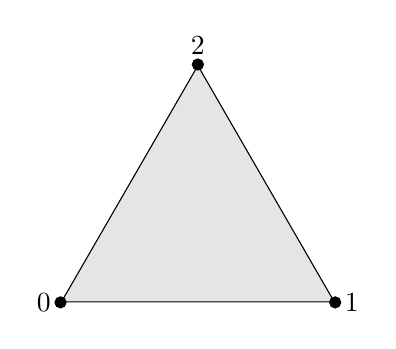
\begin{tikzpicture} % 3 nodes
      \node[name=p3, regular polygon,regular polygon sides=3, minimum size=4cm, draw, fill=black!10]{};
      \filldraw(p3.corner 1) circle (2pt);
      \filldraw(p3.corner 2) circle (2pt);
      \filldraw(p3.corner 3) circle (2pt);
      \node[above] at (p3.corner 1){2};
      \node[left] at (p3.corner 2){0};
      \node[right] at (p3.corner 3){1};
   \end{tikzpicture}
   \hspace{1cm}
   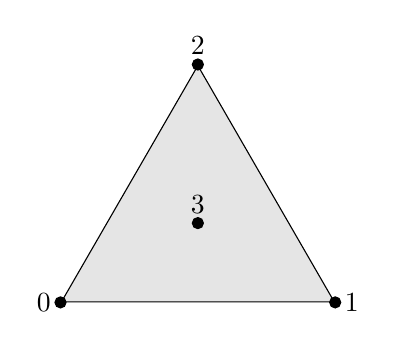
\begin{tikzpicture} % 4 nodes
      \node[name=p3, regular polygon,regular polygon sides=3, minimum size=4cm, draw,  fill=black!10]{};
      \filldraw(p3.corner 1) circle (2pt);
      \filldraw(p3.corner 2) circle (2pt);
      \filldraw(p3.corner 3) circle (2pt);
      \filldraw(p3.center) circle (2pt);
      \node[above] at (p3.corner 1){2};
      \node[left] at (p3.corner 2){0};
      \node[right] at (p3.corner 3){1};
      \node[above] at (p3.center){3};
   \end{tikzpicture}
  \end{center}
  \begin{center}  (a) \hspace{5cm} (b) \end{center}
  \begin{center}
   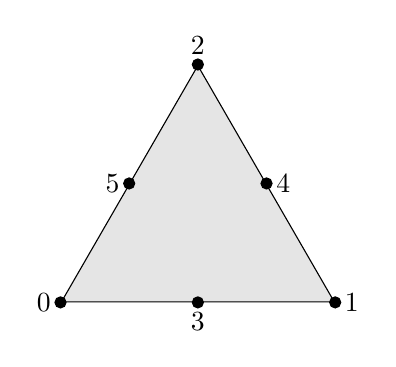
\begin{tikzpicture} % 6 nodes
      \node[name=p3, regular polygon,regular polygon sides=3, minimum size=4cm, draw,  fill=black!10]{};
      \filldraw(p3.corner 1) circle (2pt);
      \filldraw(p3.corner 2) circle (2pt);
      \filldraw(p3.corner 3) circle (2pt);
      \filldraw(p3.side 1) circle (2pt);
      \filldraw(p3.side 2) circle (2pt);
      \filldraw(p3.side 3) circle (2pt);
      \node[above] at (p3.corner 1){2};
      \node[left] at (p3.corner 2){0};
      \node[right] at (p3.corner 3){1};
      \node[left] at (p3.side 1){5};
      \node[below] at (p3.side 2){3};
      \node[right] at (p3.side 3){4};
   \end{tikzpicture}
  \end{center}
  \begin{center} (c) \end{center}

\end{document}  
